\documentclass[unicode,11pt,notheorems]{beamer}

\usepackage[T2A]{fontenc}
\usepackage[utf8]{inputenc}
\usepackage[russian]{babel}
\usepackage{amsmath,amsfonts,amssymb,amsthm}
\usepackage{colortbl,tabularx}
\usepackage{ulem}
\usepackage{tikz, graphicx}

%\usepackage{tkz-graph}
 \usetikzlibrary{positioning,arrows,calc}
\usetikzlibrary{petri}


%Описание стиля презентации
\usetheme[sidebar=0]{kfmn} 
\setbeamercovered{transparent}

%[0, 6, 8, 8, 10, 5, 6, 10, 8, 10, 10], 

\pgfdeclareimage[height=8mm]{university-logo}{logo-iem.png}
\logo{\pgfuseimage{university-logo}}
%2[0, 11, 10, 8, 11, 5, 11, 11, 8, 11, 10, 11],

\titlepicture{
	\begin{tikzpicture}[y=1.4cm,overlay,rotate=8]
	\coordinate (O) at (-3cm,0.9cm);
	\filldraw[thick,draw= vgublue, fill=vgublue!20!white] (0,0) circle[radius=4.2cm];
	\clip (0,0) circle[radius=4.2cm];
	\draw (-1.5,1.5) node{
	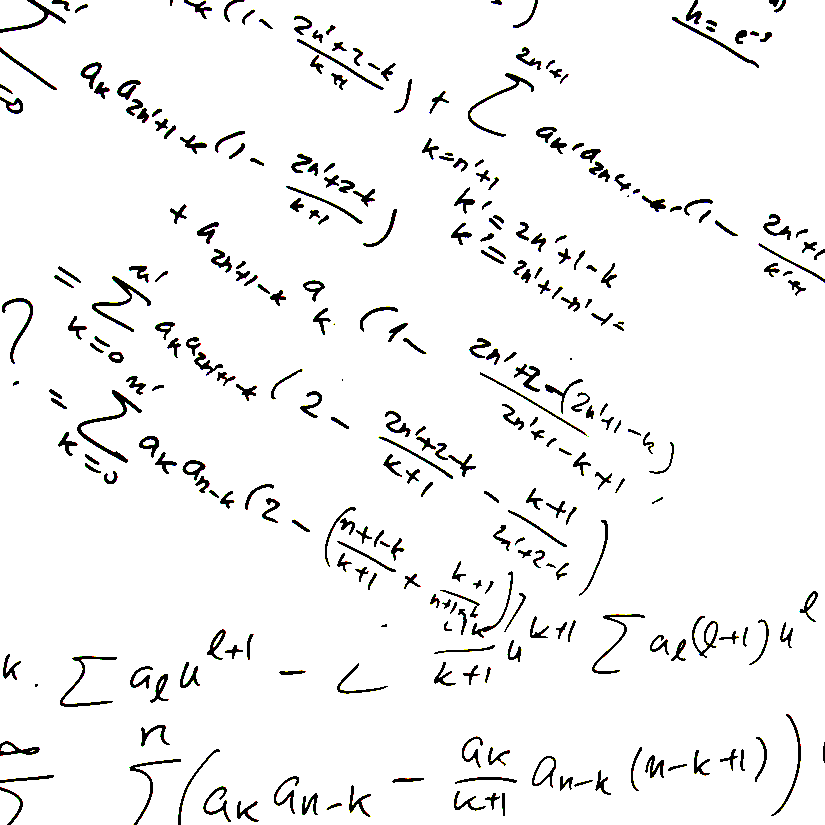
\includegraphics[width=8cm]{titlepic.png}
	};
\end{tikzpicture}
}

\usepackage[math]{iwona}

\newcommand{\hplus}{\mathbin{\hat+}}
\newcommand{\hdot}{\mathbin{\hat\cdot}}
% Описание теорем
\newtheorem{theorem}{Теорема}
\newtheorem{seq}{Следствие}
%%

%\VKR
\LECT % можно ещё лекцию забацать.
%\REPORT % можно ещё лекцию забацать.

%\titlepicture{
%%	\begin{tikzpicture}[overlay]
%%			\draw[opacity=0.4]  (-0.3,1.8) node {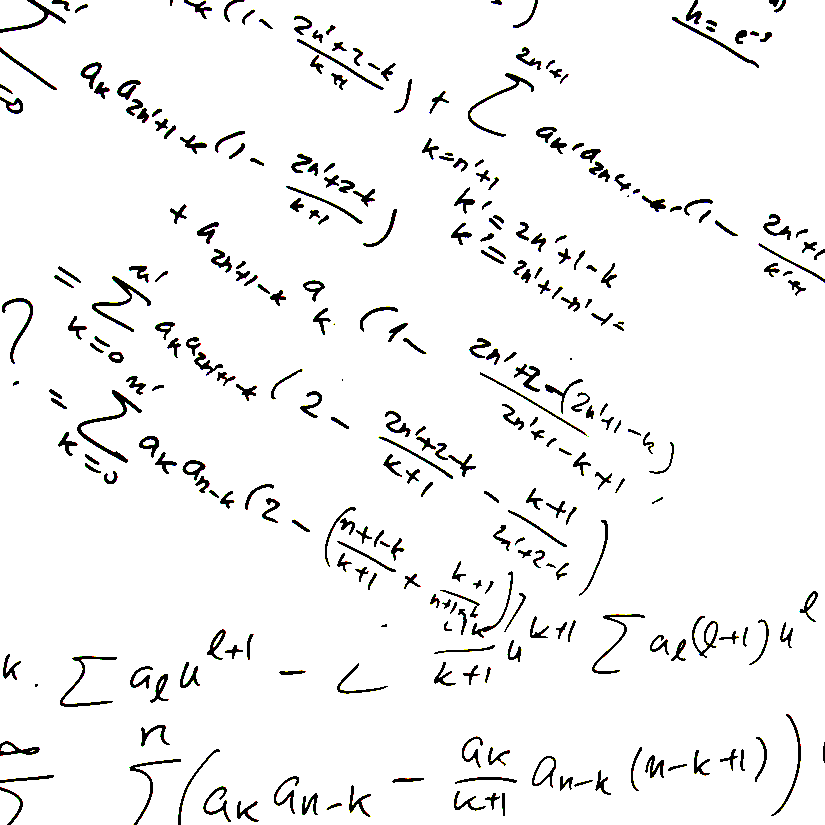
\includegraphics[width=3.5cm]{titlepic.png}};
%%	\end{tikzpicture}
%}

% Титульный лист теорем
\author[Д.\,В. Чупраков]{канд.\,физ.-матем.\,наук, доцент Д.\,В. Чупраков\\[6pt] usr10381@vyatsu.ru}

\institute[ВятГУ]{ФГБОУ ВО Вятский государственный университет}

\department{Факультет экономики и финансов}

\title[Графы и сети]{
	Введение в экономико-математическое моделирование\\[12pt]
	Лекция 1. Графы и сети}

%\subtitle{Детерминированные методы}

\date{16 апреля 2020 г.}


%\setbeamercolor{coloredboxstuff}{fg=yellow,bg=white!10!blue}

\setbeamercovered{invisible}


\tikzset{
	 myarrow/.style={->, >=latex', shorten >=1pt, thick}
}



\tikzset{add/.style n args={4}{
    minimum width=6mm,
    path picture={
        \draw[black] 
            (path picture bounding box.south east) -- (path picture bounding box.north west)
            (path picture bounding box.south west) -- (path picture bounding box.north east);
        \node at ($(path picture bounding box.south)+(0,0.13)$)     {\tiny #1};
        \node at ($(path picture bounding box.west)+(0.13,0)$)      {\tiny #2};
        \node at ($(path picture bounding box.north)+(0,-0.13)$)        {\tiny #3};
        \node at ($(path picture bounding box.east)+(-0.13,0)$)     {\tiny #4};
        }
    }
}

\tikzset{bigadd/.style n args={4}{
    minimum width=20mm,
    path picture={
        \draw[black] 
            (path picture bounding box.south east) -- (path picture bounding box.north west)
            (path picture bounding box.south west) -- (path picture bounding box.north east);
        \node at ($(path picture bounding box.south)+(0,0.5)$)     { #1};
        \node at ($(path picture bounding box.west)+(0.5,0)$)      {#2};
        \node at ($(path picture bounding box.north)+(0,-0.5)$)        {#3};
        \node at ($(path picture bounding box.east)+(-0.5,0)$)     {#4};
        }
    }
}
\begin{document}


\maketitle

\begin{frame}{Структура лекции}
	\tableofcontents
\end{frame}

\section{Введение в экономико-математическое моделирование}
\subsection{Модель и моделирование}
\begin{frame}{Понятие модели}
	\alert{Модель}~--- абстрактное представление реальности в какой-либо форме (например, в математической, физической, символической, графической или дескриптивной), предназначенное для представления определённых аспектов этой реальности и позволяющее получить ответы на изучаемые вопросы.

	\begin{block}{}
		\alert{Экономико-математическая модель} --- математическое описание экономического процесса или объекта, произведенное в целях их исследования и управления ими.
	\end{block}


	\structure{История:}
	\begin{itemize}
	\item
		Одна из первых ЭММ --- модель воспроизводства Ф. Кенэ XVIII в. 
	\item 
	 XX в. первая общая модель развивающейся экономики, Дж. фон~Нейман. 
	\end{itemize}
\end{frame}

\begin{frame}{Моделирование}
	\centering
	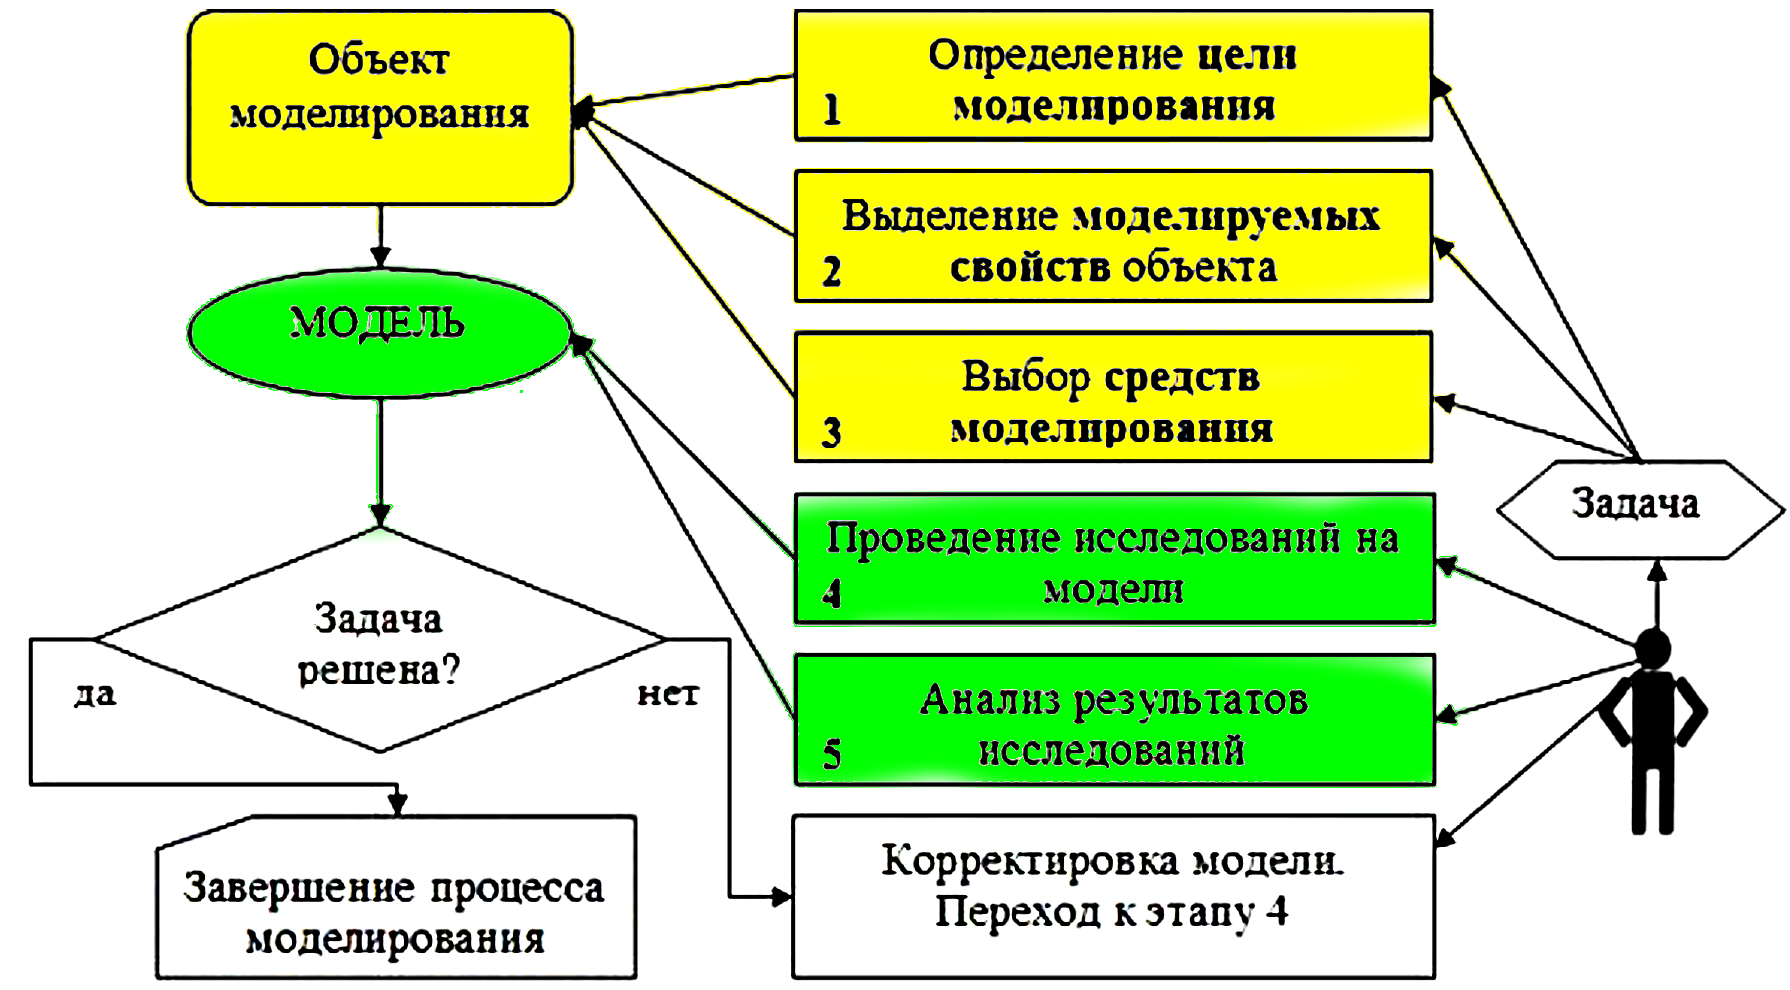
\includegraphics[width=\textwidth]{modeling.png}
\end{frame}

\subsection{Классификация моделей}

\begin{frame}{Классификация моделей}
	\centering
	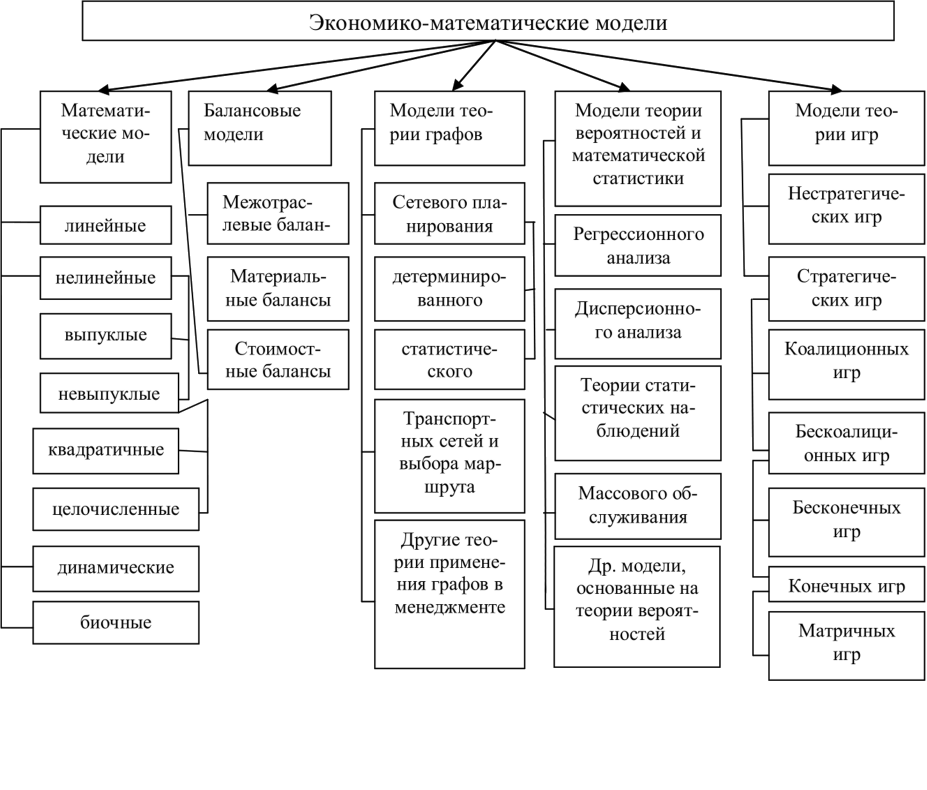
\includegraphics[width=\textwidth]{models.png}
\end{frame}

    
%    
%    Принято подразделять Э-м.м. на две большие группы:
%
%    модели, отражающие преимущественно производственный аспект экономики;
%
%    модели, отражающие преимущественно социальные аспекты экономики.
%
%    Разумеется, такое деление в значительной степени условно, поскольку в каждой из моделей в той или иной степени сочетаются производственный и социальный аспекты.
%
%    Из моделей первой группы можно назвать: модели долгосрочного прогноза сводных показателей экономического развития; межотраслевые модели; отраслевые модели оптимального планирования и размещения производства, а также модели оптимизации структуры производства   в отраслях.
%
%    Из моделей второй группы наиболее разработаны модели, связанные с прогнозированием и планированием доходов и потребления населения, демографических процессов.
%
%    Существует большое число классификаций типов Э.-м.м., которые, однако, носят фрагментарный характер. И это, по-видимому, неизбежно, так как нереально охватить все многообразие социально-экономических задач, объектов и процессов, описываемых различными моделями.
%
%    Представленные в нашем словаре модели можно условно классифицировать следующим образом
%
%    1. Наиболее общее деление моделей — по способу отражения действительности:
%
%    Аналоговая модель
%
%    Иконическая модель (то же: портретная модель)
%
%    Концептуальная модель        
%
%    Структурная модель
%
%    Функциональная модель.
%
%    2. По предназначению (цели создания и применения) модели:
%
%    Балансовая модель
%
%    Дескриптивная модель (то же: Описательная)
%
%    Имитационная модель
%
%    Информационная модель
%
%    Нормативная модель (то же: Прескриптивная модель),
%
%          в т.ч. Оптимальная модель (то же: Оптимизационная модель).
%
%    3. По способу логико-математического описания моделируемых экономических систем:
%
%    Аналитическая модель
%
%    Вероятностная модель (то же: Стохастическая модель)
%
%    Детерминированная модель
%
%    Дискретная модель
%
%    Линейная модель
%
%    Математико-статистическая модель
%
%    Матричная модель
%
%    Нелинейная модель
%
%    Непрерывная модель
%
%    Модель равновесия
%
%    Неравновесная модель
%
%    Регрессионная модель
%
%    Сетевая модель
%
%    Числовая модель
%
%    Эконометрическая модель.
%
%    - дискретного выбора
%
%    - непрерывной длительности (выживания)
%
%    -логит-иодель
%
%    -пробит-модель
%
%       -  тобит-модель..
%
%    4. По временному и пространственному признаку:
%
%    Гравитационная модель
%
%    Динамическая модель (см . Динамические модели экономики)
%
%    Модели с «бесконечным временем»
%
%    Статическая модель
%
%    Точечная модель
%
%    Трендовая модель и др..
%
%    5. По уровню моделируемого объекта в хозяйственной иерархии:
%
%    Глобальная модель
%
%    Макроэкономическая модель (то же: Агрегатная модель)
%
%    Модели мезоэкономики
%
%    Микроэкономическая модель
%
%     
%
%    6. По внутренней структуре модельного описания системы:
%
%    Автономная модель
%
%    Закрытая модель
%
%    Комплекс моделей
%
%    Многосекторная модель (многоотраслевая, многопродуктовая)
%
%    Однопродуктовая модель
%
%    Открытая модель
%
%    Система моделей (в том числе многоуровневая или многоступенчатая).
%
%    7.. По сфере применения .
%
%    Выше было указано на необозримость областей применения Э.-м.м.; поэтому мы не даем здесь их перечисления, а отсылаем к соответствующим статьям словаря: например, о прогнозных моделях — к статье Прогнозирование, об отраслевых — к статье Отраслевые задачи оптимального планирования развития и размещения производства, и т.д.
%
%    Наиболее развитая типология социально-экономических задач и моделей представлена в кн.: Вилкас Э.Й., Майминас Е.З. Решения: теория, информация, моделирование. — М.: “Радио и связь”, 1981.При разработке приведенной выше  условной классификации учитывались  материалы этой книги.
%
%Экономико-математический словарь: Словарь современной экономической науки. — М.: Дело. Л. И. Лопатников. 2003. 
%




%\subsection{О курсе}


\section{Графы и сети}
\begin{frame}{}
\centering \bfseries \Large \structure{Графы и сети}
\end{frame}

\subsection{Графы. Основные понятия}
\begin{frame}{Графы. Основные понятия}
	\begin{itemize}
	\item 
		\alert{Простой граф} $G(V, E)$~--- совокупность двух множеств
		\begin{itemize}
		\item 
			непустого множества~$V$ \alert{вершин графа};
		\item 
			множества~$E$ неупорядоченных пар различных элементов множества $V$~--- \alert{ребер графа}.
		\end{itemize}
	\item 	
		\alert{Ориентированный граф (орграф)}~--- совокупность двух множеств
				\begin{itemize}
				\item 
					непустого множества~$V$ \alert{узлов графа};
				\item 
					множества~$E$ упорядоченных пар различных элементов множества $V$~--- \alert{дуг графа}.
					Первую вершину дуги называют началом дуги, вторую~--- концом.
				\end{itemize}
	\item 	
		\alert{Взвешенный граф}~--- граф, дугам которого поставлены в соответствие некоторые значения, называемые весом (или длиной, или стоимостью) дуги 
	\item 	
		Будем считать, что в не взвешенном графе  все ребра имеют одинаковый вес~1.


\end{itemize}

%TODO Примеры графов
\end{frame}

\begin{frame}{Пути и маршруты}
	\begin{itemize}
	\item 
		\alert{Маршрут} в графе называется последовательность узлов
		и дуг вида 
		$$
			v_0, e_1, v_1, e_2, \ldots, v_{k-1}, e_k, v_k 
		$$
		так, что узел $v_{i-1}$ начало дуги $e_i$, а узел $v_i$~--- ее конец. 
	\item 
		Узел $v_0$ 	называется \alert{начальным}, а $v_k$~--- \alert{конечным} узлом пути.
	\item
		\alert{Путь}~--- это маршрут, в котором все дуги (ребра) различны. 		
	\item 
		\alert{Длина пути}~--- сумма длин (весов) тех ребер, из которых состоит путь.	
\end{itemize}

\structure{Виды путей:}
\begin{itemize}
	\item 
		Путь называется \alert{простым}, если все узлы в нем различны.
	\item 
		\alert{Цикл}~--- путь у которого начальный и конечный узлы совпадают.	
\end{itemize}

%TODO Примеры маршрутов
\end{frame}

%Лемма о цепи. Если есть цепь, соединяющая вершины u, v, то есть и простая
%цепь, соединяющая вершины u, v.


\begin{frame}{Виды графов}
\structure{Простые графы}:
\begin{itemize}

	\item 
		Простой граф называется \alert{деревом}, если он  связен и не имеет циклов.
	\item 
		\alert{Сеть}~--- орграф, не содержащий циклов, в котором ровно одна вершина имеет нулевую степень захода (\alert{коррень дерева}), и ровно одна вершина имеет нулевую степень исхода.	
\end{itemize}

\structure{Орграфы}:
\begin{itemize}
	\item Простой граф называется \alert{связным}, если любые две его вершины соединены путем


\end{itemize}
\end{frame}

\subsection{Поиск кратчайшего пути в графе}
\begin{frame}{Поиск кратчайшего пути в графе}


\begin{block}{Определение}
		Простой граф называется \alert{связным}, если любые две его вершины соединены путем
\end{block}

Для связного графа формулируется задача поиска кратчайшего пути ведется
между двумя заданными вершинами.

Ее решением является путь и его длина.

Для решения данной задачи можно использовать алгоритм, изобретённый
нидерландским ученым Э.~Дейкстрой в 1959~году.
\end{frame}
\begin{frame}{Пример }{}
Найти кратчайшие пути из вершины 1 в каждую вершину.
{\centering
\begin{tikzpicture}[>=latex]
\node[place,fill=red!20,label={[red]-120:$0$}] (P1) at (0,0) {1};
\node[place] (P2) at (3,-1) {2};
\node[place] (P3) at (2.5, 2) {3};
\node[place] (P4) at (7, 2.5) {4};
\node[place] (P5) at (4, 4) {5};
\node[place] (P6) at (0,3) {6};

\draw  (P1) -- node[above,sloped]{7} (P2);
\draw  (P1) -- node[above,sloped]{9} (P3);
\draw  (P1) -- node[above,sloped]{14} (P6);
\draw  (P2) -- node[above,sloped]{10} (P3);
\draw  (P2) -- node[above,sloped]{15} (P4);
\draw  (P3) -- node[above,sloped]{11} (P4);
\draw  (P3) -- node[above,sloped]{2} (P6);
\draw  (P4) -- node[above,sloped]{6} (P5);
\draw  (P5) -- node[above,sloped]{9} (P6);
\end{tikzpicture}
\par}
Кратчайший путь из 1 в 1 имеет длину 0. 
\end{frame}
\begin{frame}{Алгоритм Дейкстры. Шаг 1}{}

\structure{Шаг 1.} Рассмотрим всех соседей вершины~1. 

{\centering
\begin{tikzpicture}[>=latex]
	\node[place,fill=red!20, 
		  label={[red]-120:$0$}] 
		  (P1) at (0,0) {1};
	\node[place,fill=yellow!40,label={[red]-120:$7$}] 
		  (P2) at (3,-1) {2};
	\node[place,fill=yellow!40, label={[red]90:$9$}] 
		  (P3) at (2.5, 2) {3};
	\node[place] (P4) at (7, 2.5) {4};
	\node[place] (P5) at (4, 4) {5};
	\node[place,fill=yellow!40,
		  label={[red]180:$14$}] 
	      (P6) at (0,3) {6};

	\draw  (P1) -- node[above,sloped]{7} (P2);
	\draw  (P1) -- node[above,sloped]{9} (P3);
	\draw  (P1) -- node[above,sloped]{14} (P6);
	\draw  (P2) -- node[above,sloped]{10} (P3);
	\draw  (P2) -- node[above,sloped]{15} (P4);
	\draw  (P3) -- node[above,sloped]{11} (P4);
	\draw  (P3) -- node[above,sloped]{2} (P6);
	\draw  (P4) -- node[above,sloped]{6} (P5);
	\draw  (P5) -- node[above,sloped]{9} (P6);
\end{tikzpicture}
\par}
Найдем длины путей до них 	из вершины 1.

\end{frame}

\begin{frame}{Алгоритм Дейкстры. Шаг 2}{}


Вершину 1 считаем просмотренной и переходим к ее соседу c минимальной меткой~--- вершине~2.

Ее непросмотренными соседями являются вершины 3 и 4.

{\centering
\begin{tikzpicture}[>=latex]
	\node[place,fill=green!20, 
		  label={[red]-120:$0$}] 
		  (P1) at (0,0) {1};
	\node[place,fill=red!20,label={[red]-120:$7$}] 
		  (P2) at (3,-1) {2};
	\node[place,fill=yellow!40, label={[red]90:$9$}] 
		  (P3) at (2.5, 2) {3};
	\node[place,fill=yellow!40,		  		
		  label={[red]0:$22$}] 
		  (P4) at (7, 2.5) {4};
	\node[place] (P5) at (4, 4) {5};
	\node[place,
		  label={[red]180:$14$}] 
	      (P6) at (0,3) {6};

	\draw  (P1) -- node[above,sloped]{7} (P2);
	\draw  (P1) -- node[above,sloped]{9} (P3);
	\draw  (P1) -- node[above,sloped]{14} (P6);
	\draw  (P2) -- node[above,sloped]{10} (P3);
	\draw  (P2) -- node[above,sloped]{15} (P4);
	\draw  (P3) -- node[above,sloped]{11} (P4);
	\draw  (P3) -- node[above,sloped]{2} (P6);
	\draw  (P4) -- node[above,sloped]{6} (P5);
	\draw  (P5) -- node[above,sloped]{9} (P6);
	\draw[red,->,dashed]  (P2) to[out=0,in=-90] node[below,sloped]{\small $7+15=22$} (P4);
	\draw[red,->,dashed]  (P2) to[out=120,in=-100] node[below,sloped]{\small $7+10>9$} (P3);	
\end{tikzpicture}
\par}
\end{frame}

\begin{frame}{Алгоритм Дейкстры. Шаг 3}{}


Вершину 2 просмотрена. Сосед с минимальной меткой --- вершина~3.

{\centering
\begin{tikzpicture}[>=latex]
	\node[place,fill=green!20, 
		  label={[red]-120:$0$}] 
		  (P1) at (0,0) {1};
	\node[place,fill=green!20,label={[red]-120:$7$}] 
		  (P2) at (3,-1) {2};
	\node[place,fill=red!20, label={[red]90:$9$}] 
		  (P3) at (2.5, 2) {3};
	\node[place,fill=yellow!40,		  		
		  label={[red]0:\sout{$22$} $20$}] 
		  (P4) at (7, 2.5) {4};
	\node[place] (P5) at (4, 4) {5};
	\node[place,fill=yellow!40,
		  label={[red]180:$11$ \sout{$14$}}] 
	      (P6) at (0,3) {6};

	\draw  (P1) -- node[above,sloped]{7} (P2);
	\draw  (P1) -- node[above,sloped]{9} (P3);
	\draw  (P1) -- node[above,sloped]{14} (P6);
	\draw  (P2) -- node[above,sloped]{10} (P3);
	\draw  (P2) -- node[above,sloped]{15} (P4);
	\draw  (P3) -- node[above,sloped]{11} (P4);
	\draw  (P3) -- node[above,sloped]{2} (P6);
	\draw  (P4) -- node[above,sloped]{6} (P5);
	\draw  (P5) -- node[above,sloped]{9} (P6);
	\draw[red,->,dashed]  (P3) to[out=-20,in=-160] node[below,sloped]{\small $9+11=20<22$} (P4);
	\draw[red,->,dashed]  (P3) to[out=-160,in=-60] node[below,sloped]{\small $9+2=11<14$} (P6);	
%	\draw[red,->,dashed]  (P2) to[out=120,in=-100] node[below,sloped]{7+10>9} (P3);	
\end{tikzpicture}
\par}
\end{frame}

\begin{frame}{Алгоритм Дейкстры. Шаг 4}{}


Вершина 3 просмотрена. Ее сосед с минимальной меткой --- вершина~6.

{\centering
\begin{tikzpicture}[>=latex]
	\node[place,fill=green!20, 
		  label={[red]-120:$0$}] 
		  (P1) at (0,0) {1};
	\node[place,fill=green!20,label={[red]-120:$7$}] 
		  (P2) at (3,-1) {2};
	\node[place,fill=green!20, label={[red]90:$9$}] 
		  (P3) at (2.5, 2) {3};
	\node[place,
		  label={[red]0: $20$}] 
		  (P4) at (7, 2.5) {4};
	\node[place,fill=yellow!40,
		  label={[red]90:$20$}] (P5) at (4, 4) {5};
	\node[place,fill=red!20,
		  label={[red]180:$11$}]
	      (P6) at (0,3) {6};

	\draw  (P1) -- node[above,sloped]{7} (P2);
	\draw  (P1) -- node[above,sloped]{9} (P3);
	\draw  (P1) -- node[above,sloped]{14} (P6);
	\draw  (P2) -- node[above,sloped]{10} (P3);
	\draw  (P2) -- node[above,sloped]{15} (P4);
	\draw  (P3) -- node[above,sloped]{11} (P4);
	\draw  (P3) -- node[above,sloped]{2} (P6);
	\draw  (P4) -- node[above,sloped]{6} (P5);
	\draw  (P5) -- node[above,sloped]{9} (P6);
	\draw[red,->,dashed]  (P6) to[out=40,in=170] node[above,sloped]{\small $11+9=20$} (P5);
%	\draw[red,->,dashed]  (P2) to[out=120,in=-100] node[below,sloped]{7+10>9} (P3);	
\end{tikzpicture}
\par}
\end{frame}

\begin{frame}{Алгоритм Дейкстры. Шаг 5}{}
Вершина 6 просмотрена. Ее сосед с минимальной меткой --- вершина~5.

{\centering
\begin{tikzpicture}[>=latex]
	\node[place,fill=green!20, 
		  label={[red]-120:$0$}] 
		  (P1) at (0,0) {1};
	\node[place,fill=green!20,label={[red]-120:$7$}] 
		  (P2) at (3,-1) {2};
	\node[place,fill=green!20, label={[red]90:$9$}] 
		  (P3) at (2.5, 2) {3};
	\node[place, fill=yellow!40,
		  label={[red]0: $20$}] 
		  (P4) at (7, 2.5) {4};
	\node[place,fill=red!20,
		  label={[red]90:$20$}] (P5) at (4, 4) {5};
	\node[place,fill=green!20,
		  label={[red]180:$11$}]
	      (P6) at (0,3) {6};

	\draw  (P1) -- node[above,sloped]{7} (P2);
	\draw  (P1) -- node[above,sloped]{9} (P3);
	\draw  (P1) -- node[above,sloped]{14} (P6);
	\draw  (P2) -- node[above,sloped]{10} (P3);
	\draw  (P2) -- node[above,sloped]{15} (P4);
	\draw  (P3) -- node[above,sloped]{11} (P4);
	\draw  (P3) -- node[above,sloped]{2} (P6);
	\draw  (P4) -- node[above,sloped]{6} (P5);
	\draw  (P5) -- node[above,sloped]{9} (P6);
	\draw[red,->,dashed]  (P5) to[out=0,in=120] node[above,sloped]{\small $20+6=26>20$} (P4);
%	\draw[red,->,dashed]  (P2) to[out=120,in=-100] node[below,sloped]{7+10>9} (P3);	
\end{tikzpicture}
\par}
\end{frame}
\begin{frame}{Алгоритм Дейкстры. Шаг 6. Завершение}{}


Вершина 5 просмотрена. Ее сосед с минимальной меткой --- вершина~4.
У которой, в свою очередь, нее нет не просмотренных соседей.

{\centering
\begin{tikzpicture}[>=latex]
	\node[place,fill=green!20, 
		  label={[red]-120:$0$}] 
		  (P1) at (0,0) {1};
	\node[place,fill=green!20,label={[red]0:$7$}] 
		  (P2) at (3,-1) {2};
	\node[place,fill=green!20, label={[red]90:$9$}] 
		  (P3) at (2.5, 2) {3};
	\node[place, fill=red!20,
		  label={[red]0: $20$}] 
		  (P4) at (7, 2.5) {4};
	\node[place,fill=green!20,
		  label={[red]90:$20$}] (P5) at (4, 4) {5};
	\node[place,fill=green!20,
		  label={[red]180:$11$}]
	      (P6) at (0,3) {6};

	\draw  (P1) -- node[above,sloped]{7} (P2);
	\draw  (P1) -- node[above,sloped]{9} (P3);
	\draw  (P1) -- node[above,sloped]{14} (P6);
	\draw  (P2) -- node[above,sloped]{10} (P3);
	\draw  (P2) -- node[above,sloped]{15} (P4);
	\draw  (P3) -- node[above,sloped]{11} (P4);
	\draw  (P3) -- node[above,sloped]{2} (P6);
	\draw  (P4) -- node[above,sloped]{6} (P5);
	\draw  (P5) -- node[above,sloped]{9} (P6);
\end{tikzpicture}
\par}
\end{frame}
\begin{frame}{Кратчайшие пути из вершины 1}{}

Из вершины 1 имеются следующие кратчайшие пути:

\medskip
{\centering
\begin{tabular}{ccc}
\hline
\structure{Вершина} & \structure{Длина пути} & \structure{Путь}\\
\hline
2 & 7& (1,2)\\
3 & 9& (1,3) \\
4 & 20& (1,3,4)\\
5 & 20& (1,3,6,5)\\
6 & 11& (1,3,6)\\
\hline
\end{tabular}
\par}
\end{frame}

\subsection{Дерево решений}
\begin{frame}{Дерево решений}
	\begin{block}{Определение}
		Простой граф называется \alert{деревом}, если он  связен и не имеет циклов.
		\begin{itemize}
		\item 
			  Одну выделенную вершину, называют \alert{корнем дерева}.
		\item 
			Вершины степени~1 называются \alert{листьями дерева}.
		\end{itemize}
	\end{block}

	\medskip
	\structure{Идея метода:} Представлении последовательности стратегических решений в виде дерева, где каждое решение и каждое событие становится точкой ветвления.


	
	Пути от корня к листьям показывают возможные стратегии развития моделируемой системы.

	\medskip
	\structure{Область применения:} принятие решений  в условиях риска.  
	
\end{frame}

\begin{frame}{Основные элементы дерева решений}
\begin{itemize}
\item 
	Выделяются два вида вершин:
	\begin{itemize}
	\item квадраты~--- моменты принятия решений, 
	\item круги --- моменты случайных событий --- рисков. 	
	\end{itemize}
\item 
	Ветви, исходящие из квадратных узлов, обозначают варианты решений.
\item 
	Ветви, исходящие из круглых узлов, --- возможные события.
\end{itemize}
\end{frame}
\begin{frame}{Принцип построения дерева решений}
\begin{itemize}
\item
	Дерево «выстраивается» слева направо. 
\item 
	Все моменты принятия решений упорядочиваются хронологически.
\item 
	Корнем является самый ранний момент принятия решения.
\item 
	От каждого квадрата отходят ребра к кругам- обозначающим события, которые возможны при выбранном варианте решения.
\item 
	От каждого круга отходят ребра к квадратам являющимся характеризующими момент реакции на событие.
\item 
	Процесс построения дерева продвигается вперед по времени через ряд последовательных решений и событий до тех пор, пока все логические последовательности и вытекающие из них отдачи не будут вычерчены.
\end{itemize}
\end{frame}
%	\begin{itemize}
%	\item
%		Дерево «выстраивается» слева направо. 
%	\item 
%		После того как дерево решения построено, оно анализируется справа налево, т.е. начинать надо с последнего принятого решения. 
%	\item 
%		Для каждого решения выбирается альтернатива с наибольшим показателем отдачи (или с наименьшими затратами). 
%	\item 
%		Если за принятием решения следует несколько возможных вариантов событий, выбирают альтернативу с наибольшей предполагаемой прибылью (или с наименьшей предполагаемой величиной затрат).
%\end{itemize}
%\end{frame}

\begin{frame}{Кейс}
	Рассматривается проект инвестирования \textbf{7~млн. руб.} в~разработку новой технологии.
	\begin{itemize}
	\item 
		По предварительным оценкам технология будет востребована с вероятностью \textbf{0.6}. 
		В этом случае инвестиции принесут доход \textbf{12 млн. руб.}
		Если же технология будет не востребована, то доход составит \textbf{0 рублей.}

	\item 
		Через неделю будет опубликован аналитический прогноз аналитической фирмы относительно востребованности технологии.
		Надежность прогноза эксперты оценивают в \textbf{0,7}.
	\item 
		Однако, в случае положительного прогноза пакет порождает до \textbf{10,6 млн. руб}, а в случае отрицательного подешевеет до \textbf{3,4 млн. руб}
\end{itemize}
\alert{Какой стратегии лучше придерживаться: инвестировать сейчас или ждать прогноза?
Стоит ли инвестировать при том или ином результате прогноза? }
\end{frame}

\begin{frame}{Формализация}
	\structure{Моменты принятия решений:}
	\begin{itemize}
	\item 
		Начальный момент: инвестировать или ждать прогноза.
	\item 
		После опубликования прогноза: инвестировать или нет
	\end{itemize}

	Моменты принятия решений:
	\begin{itemize}
	\item 
		Начальный момент: инвестировать или ждать прогноза.
	\item 
		После опубликования прогноза: инвестировать или нет
	\end{itemize}

\end{frame}


\begin{frame}{Дерево решений}{}
{\centering
\begin{tikzpicture}[>=latex]
%	\draw[lightgray] (-1,1)-- +(10,0);
%	\foreach \x in {-1,1,...,9}
%		\draw[lightgray] (\x,2)-- +(0,-5);
%	\foreach \x in {0,1,...,4}
%		\draw (2*\x,1.5) node {\x};

\node[transition,fill=yellow] (T0) at (0,0) {};
\node[transition,fill=yellow] (T11) at (4,-1) {};
\node[transition,fill=yellow] (T12) at (4,-3) {};

\node[place,fill=red!30] (Predict) at (2,-2) {Пр};
\node[place,fill=red!30] (Invest) at (2,3) {};
\node[place,fill=red!30] (Invest2) at (6,0) {};
\node[place,fill=red!30] (Invest3) at (6,-2) {};


\node[transition,fill=green!30] (LWin1) at (8,3) {12};
\node[transition,fill=green!30] (LLose1) at (8,2) {0};
\node[transition,fill=green!30] (LWin2) at (8,1) {12};
\node[transition,fill=green!30] (LLose2) at (8,0) {0};
\node[transition,fill=green!30] (LDeny2) at (8,-1) {0};
\node[transition,fill=green!30] (LDeny3) at (8,-4) {0};
\node[transition,fill=green!30] (LWin3) at (8,-2) {12};
\node[transition,fill=green!30] (LLose3) at (8,-3) {0};

\node (LWin1Delta) at (9,3) {$5$};
\node (LLose1Delta) at (9,2) {$-7$};
\node (LWin2Delta) at (9,1) {$1.4$};
\node (LLose2Delta) at (9,0) {$-10.6$};
\node (LDeny2Delta) at (9,-1) {$0$};
\node (LDeny3Delta) at (9,-4) {$0$};
\node (LWin3Delta) at (9,-2) {$8.6$};
\node (LLose3Delta) at (9,-3) {$-3.4$};


\draw  (T0) 
		-- node[above,sloped]{\scriptsize инвестируем} 
		   node[below,sloped]{\scriptsize $-7$} 
		(Invest);
\draw  (T0) -- node[above,sloped]{\scriptsize ждем} (Predict);
\draw  (Predict) -- node[above,sloped]{\scriptsize $+$} (T11);
\draw  (Predict) -- node[below,sloped]{\scriptsize $-$} (T12);
\draw  (T11) 
		-- node[above,sloped]{\scriptsize инвестируем} 
	   	   node[below,sloped]{\scriptsize $-10.6$} (Invest2);
\draw  (T11) -- node[above,sloped]{\scriptsize нет} (LDeny2);
\draw  (T12) 
		-- node[above,sloped]{\scriptsize инвестируем} 
 		   node[below,sloped]{\scriptsize $-3.4$} (Invest3);
\draw  (T12) -- node[above,sloped]{\scriptsize нет} (LDeny3);
\draw  (Invest) 
		-- node[above,sloped]{\scriptsize востр.} 
		   node[below,sloped]{\scriptsize $0.6$} (LWin1);
\draw  (Invest) 
	|- node[pos=0.8,above,sloped]{\scriptsize нет} 
	   node[pos=0.8,below,sloped]{\scriptsize $0.4$}
	(LLose1);

\draw  (Invest2) 
	|- node[pos=0.8,above,sloped]{\scriptsize верен} 
	   node[pos=0.8,below,sloped]{\scriptsize $0.7$} (LWin2);
\draw  (Invest2) 
	-- node[above,sloped]{\scriptsize нет} 
	   node[below,sloped]{\scriptsize $0.3$} (LLose2);

\draw  (Invest3) 
	|- node[pos=0.8,above,sloped]{\scriptsize верен} 
	   node[pos=0.8,below,sloped]{\scriptsize $0.7$} (LLose3);
\draw  (Invest3) 
	-- node[above,sloped]{\scriptsize нет} 
	   node[below,sloped]{\scriptsize $0.3$} (LWin3);
\end{tikzpicture}
\par}
\end{frame}

\begin{frame}{Анализ дерева решений}{}
\noindent\begin{tabular}{ll}
\hline
\structure{Стратегии} & \structure{Ожидаемый доход}\\
\hline
Инвестировать сразу: & $5\cdot 0.6-7\cdot 0.4 = \alert{0.20}$\\
Инвестировать, если прогноз $(+)$: & $1.4\cdot 0.7-10.4\cdot 0.3 = -2.14$\\
Инвестировать, если прогноз $(-)$: & $-3.4\cdot 0.7+8.6 \cdot 0.3 = \alert{0.20}$\\
\hline
\end{tabular}

\medskip
Инвестиция сразу столь же выгодна в среднем, как и инвестиция в случае отрицательного прогноза. Однако отсутствует риск положительного прогноза.

\medskip
\alert{Оптимальный план --- незамедлительная инвестиция.}


\end{frame}

\subsection{Сетевая модель}

\begin{frame}{Сетевая модель}
	\alert{Сетевая модель} --- изображение плана выполнения комплекса работ в виде связного орграфа, отражающего последовательность и зависимость выполняемых операций.


	\structure{Область применения:}
	\begin{itemize}
	\item 
		Формирование календарного плана реализации комплекса работ.
	\item 
		Принятие эффективных решений в процессе выполнения этого плана.
	\end{itemize}

	\structure{Достоинства:}
	\begin{itemize}
	\item 
		Наглядность.
	\item 
		Инструмент для разделения полномочий и ответственности за выполнение работ.
	\item 
		\alert{Можно и нужно  применять для организации собственной деятельности уже сейчас!}
	\end{itemize}

%	\structure{Суть метода:}
%	Группа экспертов дает свою оценку всем направлениям и вариантам решения проблемы, выделяя наиболее приоритетный путь (вариант). Показывает «пробелы», которым не уделили внимания. 
\end{frame}

\begin{frame}{Элементы сетевой модели}
~
{\centering
\begin{tikzpicture}[>=latex,]
\node[place] (P0) {0};
\node[place] (P1) [above right=of P0] {1};
\node[place] (P2) [below right=of P0] {2};
\node[place] (P3) [right=of P1] {3};
\node[place] (P4) [right=of P2] {4};
\node[place] (P5) [below right=of P3] {5};
\draw [->] (P0) -- node[above,sloped]{5} (P1);
\draw [->] (P0) -- node[above,sloped]{2} (P2);
\draw [dashed,->] (P1) -- (P2);
\draw [->] (P1) -- node[above,sloped]{3}  (P3);
\draw [->] (P2) -- node[above,sloped]{6}  (P3);
\draw [->] (P2) -- node[above,sloped]{6} (P4);
\draw [->] (P3) -- node[above,sloped]{4} (P5);
\draw [->] (P4) -- node[above,sloped]{5} (P5);
\end{tikzpicture}
\par}

\alert{События}~--- узлы орграфа 
	\begin{itemize}
	\item 0 --- исходное событие 
	\item 5 --- завершающее событие 
	\end{itemize}

\alert{Работы}~--- дуги орграфа. Вес дуги --- продолжительность работы.
	\begin{itemize}
	\item (0,1)~--- работа, продолжительностью 5~единиц.
	\item (1,2) --- фиктивная работа, продолжительность 0~единиц.
	\end{itemize}
	
\end{frame}


\begin{frame}{Элементы сетевой модели. Работы}

\begin{block}{Определение}
	\alert{Работа}~--- совокупность приемов и действий, необходимых для выполнения конкретной задачи или достижения определенной цели. 
\end{block}
	\structure{Виды работ:}
	\begin{itemize}
	\item 
		\alert{Работа-действие}~--- процесс, требующий затрат времени и ресурсов. 

	\item 
		\alert{Работа-ожидание}~--- процесс, требующий затрат времени, но не требующий ресурсных затрат. 

	\item 
		\alert{Зависимость (фиктивная работа)}~---  не требует ни затрат времени ни затрат ресурсов.
		Упорядочивает связываемые ей состояния. 
		

	\end{itemize}

	\medskip
%	\structure{Изображение на графе:}
	
	\alert{Работы} изображаются дугами орграфа.
	\begin{itemize}
	\item 
		Работа-действие и работа-ожидание~--- сплошная линия;
	\item 
		Зависимость~---пунктирная линия.
	\end{itemize}

\end{frame}

\begin{frame}{Правила построения  сетевой модели}
	\begin{itemize}
	\item
		В сетевом графике не должно быть «тупиковых» событий, то есть событий, из которых не выходит ни одна работа, за исключением завершающего события.
	\item
		В сетевом графике не должно быть «хвостовых» событий, то есть событий, которым не предшествует хотя бы одна работа, за исключением исходного.
	\item
		В нем не должно быть циклов.
	\item
		Любые два события должны быть непосредственно связаны не более чем одной работой.
	\item
		В сети рекомендуется иметь одно исходное и одно завершающее событие.
	\item
		Сетевой график должен быть упорядочен. То есть события и работы должны располагаться так, чтобы для любой работы предшествующее ей событие было расположено левее и имело меньший номер по сравнению с завершающим эту работу событием.		
	\end{itemize}
\end{frame}

\begin{frame}{Упорядочение событий}

Каждому событию~$I$ сопоставляется \alert{ранг}~--- максимальное число дуг пути от исходного события к событию $I$.	

{\centering
\begin{tikzpicture}[>=latex]
	\draw[lightgray] (-1,1)-- +(10,0);
	\foreach \x in {-1,1,...,9}
		\draw[lightgray] (\x,2)-- +(0,-5);
	\foreach \x in {0,1,...,4}
		\draw (2*\x,1.5) node {\x};

\node[place] (P0) at (0,-1) {0};
\node[place] (P1) at (2,0) {1};
\node[place] (P2) at (4,-2) {2};
\node[place] (P3) at (6,0) {3};
\node[place] (P4) at (6,-2) {4};
\node[place] (P5) at (8,-1) {5};
\draw [->] (P0) -- node[above,sloped]{5} (P1);
\draw [->] (P0) -- node[above,sloped]{2} (P2);
\draw [dashed,->] (P1) -- (P2);
\draw [->] (P1) -- node[above,sloped]{3}  (P3);
\draw [->] (P2) -- node[above,sloped]{6}  (P3);
\draw [->] (P2) -- node[above,sloped]{6} (P4);
\draw [->] (P3) -- node[above,sloped]{4} (P5);
\draw [->] (P4) -- node[above,sloped]{5} (P5);
\end{tikzpicture}
\par}

	Нумерация событий выполняется следующим образом:
	\begin{itemize}
	\item 
		большему рангу соответствует больший номер события;
	\item 
		события, с одинаковым рангом, нумеруются произвольно.
	\end{itemize}
\end{frame}





\begin{frame}{Временн\'{ы}е параметры событий}
	\begin{itemize}
	\item[$t_\text{р}(i)$]~--- 
		ранний (ожидаемый) срок свершения $i$-го события: 
		$$\alert{t_\text{р}(i) = \max\limits_{j}\big(t_\text{р}(j)+t(j,i)\big)}$$

	\item[$t_\text{п}(i)$]~--- 
		поздний (предельный) срок: 
		$$\alert{t_\text{п}(i) = \min\limits_{j}\big(t_\text{п}(j)-t(i,j)\big)}$$
 	
	\item[$R(i)$]~--- 			
		резерв времени  i-го события:
		$$\alert{R(i)=t_\text{п}(i) - t_\text{р}(i)}$$
	\end{itemize}

	\structure{Изображение события:}\quad
\begin{tikzpicture}[baseline]
	\node[minimum height=2cm,draw,circle,bigadd={$i$}{$t_\text{р}(i)$}{$R(i)$}{$t_\text{п}(i)$}] (P0) at (0,0) {};
\end{tikzpicture}
\end{frame}
%	\medskip
%	\structure{Частные случаи:}
%	\begin{itemize}
%	\item ранний и поздний сроки свершения исходного события~--- 0
%	
%	\item поздний срок свершения завершающего события~--- продолжительность  критического пути.
%
%%	\item[$t_\text{п}(i)$]~--- 
%%		поздний (предельный) срок: 
%%		$t_\text{п}(i) = \min\limits_{i,j}(t_\text{п}(j)-t(i,j))$.
%% 	
%%	\item[$R(i)$]~--- 			
%%		резерв времени  i-го события:
%%		$R(i)=t_\text{п}(i) - t_\text{р}(i)$
%	\end{itemize}


\begin{frame}{Вычисление временных параметров событий}


Ранний срок свершения событий вычисляется \alert{слева направо}:
{\centering
\begin{tikzpicture}[>=latex]
	\node[draw,circle,add={0}{0}{0}{0}] (P0) at (0,-1) {};
	\node[draw,circle,add={1}{5}{}{}] (P1) at (2,0) {};
	\node[draw,circle,add={2}{5}{}{}] (P2) at (4,-2) {};
	\node[draw,circle,add={3}{11}{}{}] (P3) at (6,0) {};
	\node[draw,circle,add={4}{11}{}{}] (P4) at (6,-2) {};
	\node[draw,circle,add={5}{16}{}{}] (P5) at (8,-1) {};
	\draw [->,red,thick] (P0) -- node[above,sloped]{5} (P1);
	\draw [->] (P0) -- node[above,sloped]{2} (P2);
	\draw [dashed,->,red,thick] (P1) --node[above,sloped]{0} (P2);
	\draw [->] (P1) -- node[above,sloped]{3}  (P3);
	\draw [->,red,thick] (P2) -- node[above,sloped]{6}  (P3);
	\draw [->,red,thick] (P2) -- node[above,sloped]{6} (P4);
	\draw [->] (P3) -- node[above,sloped]{4} (P5);
	\draw [->,red,thick] (P4) -- node[above,sloped]{5} (P5);
\end{tikzpicture}

\vspace{1cm}
Поздний срок свершения событий вычисляется \alert{справа налево}:
\begin{tikzpicture}[>=latex]
	\node[draw,circle,add={0}{0}{0}{0}] (P0) at (0,-1) {};
	\node[draw,circle,add={1}{5}{0}{5}] (P1) at (2,0) {};
	\node[draw,circle,add={2}{5}{0}{5}] (P2) at (4,-2) {};
	\node[draw,circle,add={3}{11}{1}{12}] (P3) at (6,0) {};
	\node[draw,circle,add={4}{11}{0}{11}] (P4) at (6,-2) {};
	\node[draw,circle,add={5}{16}{0}{16}] (P5) at (8,-1) {};
	\draw [->,blue,thick] (P0) -- node[above,sloped]{5} (P1);
	\draw [->] (P0) -- node[above,sloped]{2} (P2);
	\draw [dashed,->,blue,thick] (P1) --node[above,sloped]{0} (P2);
	\draw [->] (P1) -- node[above,sloped]{3}  (P3);
	\draw [->] (P2) -- node[above,sloped]{6}  (P3);
	\draw [->,blue,thick] (P2) -- node[above,sloped]{6} (P4);
	\draw [->,blue,thick] (P3) -- node[above,sloped]{4} (P5);
	\draw [->,blue,thick] (P4) -- node[above,sloped]{5} (P5);
\end{tikzpicture}

\par}

\end{frame}


\begin{frame}{Критический путь}
	\begin{itemize}
	\item
		\alert{Полный путь}~--- это путь, соединяющий исходное событие с завершающим.
	\item
		\alert{Критический путь}~--- полный путь наибольшей длины.
	\end{itemize}
	
\begin{tikzpicture}[>=latex]
	\node[draw,circle,add={0}{0}{0}{0}] (P0) at (0,-1) {};
	\node[draw,circle,add={1}{5}{0}{5}] (P1) at (2,0) {};
	\node[draw,circle,add={2}{5}{0}{5}] (P2) at (4,-2) {};
	\node[draw,circle,add={3}{11}{1}{12}] (P3) at (6,0) {};
	\node[draw,circle,add={4}{11}{0}{11}] (P4) at (6,-2) {};
	\node[draw,circle,add={5}{16}{0}{16}] (P5) at (8,-1) {};
	\draw [->,red,thick] (P0) -- node[above,sloped]{5} (P1);
	\draw [->] (P0) -- node[above,sloped]{2} (P2);
	\draw [dashed,->,red,thick] (P1) --node[above,sloped]{} (P2);
	\draw [->] (P1) -- node[above,sloped]{3}  (P3);
	\draw [->] (P2) -- node[above,sloped]{6}  (P3);
	\draw [->,red,thick] (P2) -- node[above,sloped]{6} (P4);
	\draw [->] (P3) -- node[above,sloped]{4} (P5);
	\draw [->,red,thick] (P4) -- node[above,sloped]{5} (P5);
\end{tikzpicture}	
\begin{block}{Теорема}
\itshape Все вершины, лежащие на критическом пути имеют нулевой резерв времени.
\end{block}
\end{frame}

%\begin{frame}{Временн\'{ы}е параметры работ}
%	\begin{itemize}
%	\item[$t_\text{рн}(i,j)$]~--- 
%		ранний срок начала работы $i,j$: 
%		$\alert{t_\text{рн}(i,j)=t_\text{р}(i)}$
%
%	\item[$t_\text{ро}(i,j)$]~--- 
%		ранний срок окончания работы $i,j$: 
%		$\alert{t_\text{ро}(i,j)=t_\text{р}(i)+t(i,j)}$
%
%	\item[$t_\text{пн}(i,j)$]~--- 
%		поздний срок начала работы $i,j$: 
%		$\alert{t_\text{пн}(i,j)=t_\text{п}(i)-t(i,j)}$
%
%	\item[$t_\text{по}(i,j)$]~--- 
%		поздний срок окончания работы $i,j$: 
%		$\alert{t_\text{по}(i,j)=t_\text{п}(о)}$
%
%	\item[$R_\text{п}(i,j)$]~--- 	полный резерв времени  работы $(i,j)$:		
%		$$\alert{R_\text{п}(i,j)= t_\text{п}(j) - t_\text{р}(i)-t(i,j)}$$
%	\end{itemize}
%\end{frame}

\section{Резюме лекции и домашнее задание}
\begin{frame}{Резюме}
В ходе лекции изучены три модели:
	\begin{itemize}
		\item графовая модель;
		\item дерево решений;
		\item сетевой график.
	\end{itemize}		

\medskip
	После проработки лекции вы должны уметь:
	\begin{itemize}
	\item 
		представлять моделируемые системы в виде графов;
	\item 
		находить кратчайший путь в графе;
	\item 
		выбирать оптимальное решение из конечного множества в условиях риска;
	\item 
		строить сетевой график выполнения этих работ;
	\item 
		находить критические пути и их продолжительность;
	\item 
		рассчитывать временные характеристики сетевого графика, выявлять узкие места;
	\end{itemize}		
\end{frame}


\begin{frame}{Задание}
Для завершения лекции вам необходимо подготовить конспект, в который должны войти:
	\begin{enumerate}
		\item 
			 Не менее двух определений экономико-математической модели (с указанием первоисточника определения).
		\item 
			 Классификация экономико-математических моделей.
		\item 
			 Основные понятия графов.
		\item 
			  Этапы моделирования.
		\item 
			 Алгоритм Дейкстры в форме последовательности действий.
		\item 
			 Алгоритм построения дерева решений.
		\item 
			 Построение линейной диаграммы проекта 
		\item 
			 Пример расчета временных параметров и их значение.
		\item 
			 Алгоритм нахождения критического пути.
	\end{enumerate}

Конспект

\end{frame}
\begin{frame}{Источники информации}
\begin{itemize}
\item 
	Сетевые модели:  {\color{blue}\href{https://cloud.mail.ru/public/4SN3/2MJYgEz95}{Кремер  Н.\,Ш. Исследование операций в экономике}} Глава 14, с. 286--311.
	\begin{itemize}
		\item  
			Построение линейной диаграммы проекта: c. 288
		\item 
			 Расчет временных параметров и поиск критического пути:  c. 299--311
	\end{itemize}
\item 
	Классификация экономико-математических моделей: 	
	{\color{blue}\href{https://cloud.mail.ru/public/4WWa/4qH2ceM1H}{Панкратов Е.\,Л., Булаева Е.\,А., Болдыревский П.\,Б. Ведение в экономико-математическое моделирование. Учебное пособие. --- Нижний Новгород: Нижегородский госуниверситет, 2017. }} c. 5--10.
\item Все материалы по курсу будут здесь:
{\color{blue}\url{https://cloud.mail.ru/public/48BX/47oESuaQQ}}

\end{itemize}

\end{frame}

\begin{frame}{Анонс:}
	На следующей лекции мы научимся:
	\begin{itemize}
	\item 
		определять стратегию минимального удорожания комплекса работ при сокращении  сроков;
	\item 
		определять коэффициенты напряженности работ;
	\item 
		оценивать вероятность того, что фактический срок выполнения проекта не превзойдет заданного директивного срока;
	\item 
		определять максимальный срок выполнения проекта, который возможен с заданной надежностью.	
	\end{itemize}

\end{frame}
\end{document}



